\section{Диаграмма вариантов использования}
На рисунке \ref{use_case} представленна Use Case диаграмма сценариев использования с описанными ранее видами акторов.


\begin{figure}[ph!]
	\begin{center}
%		{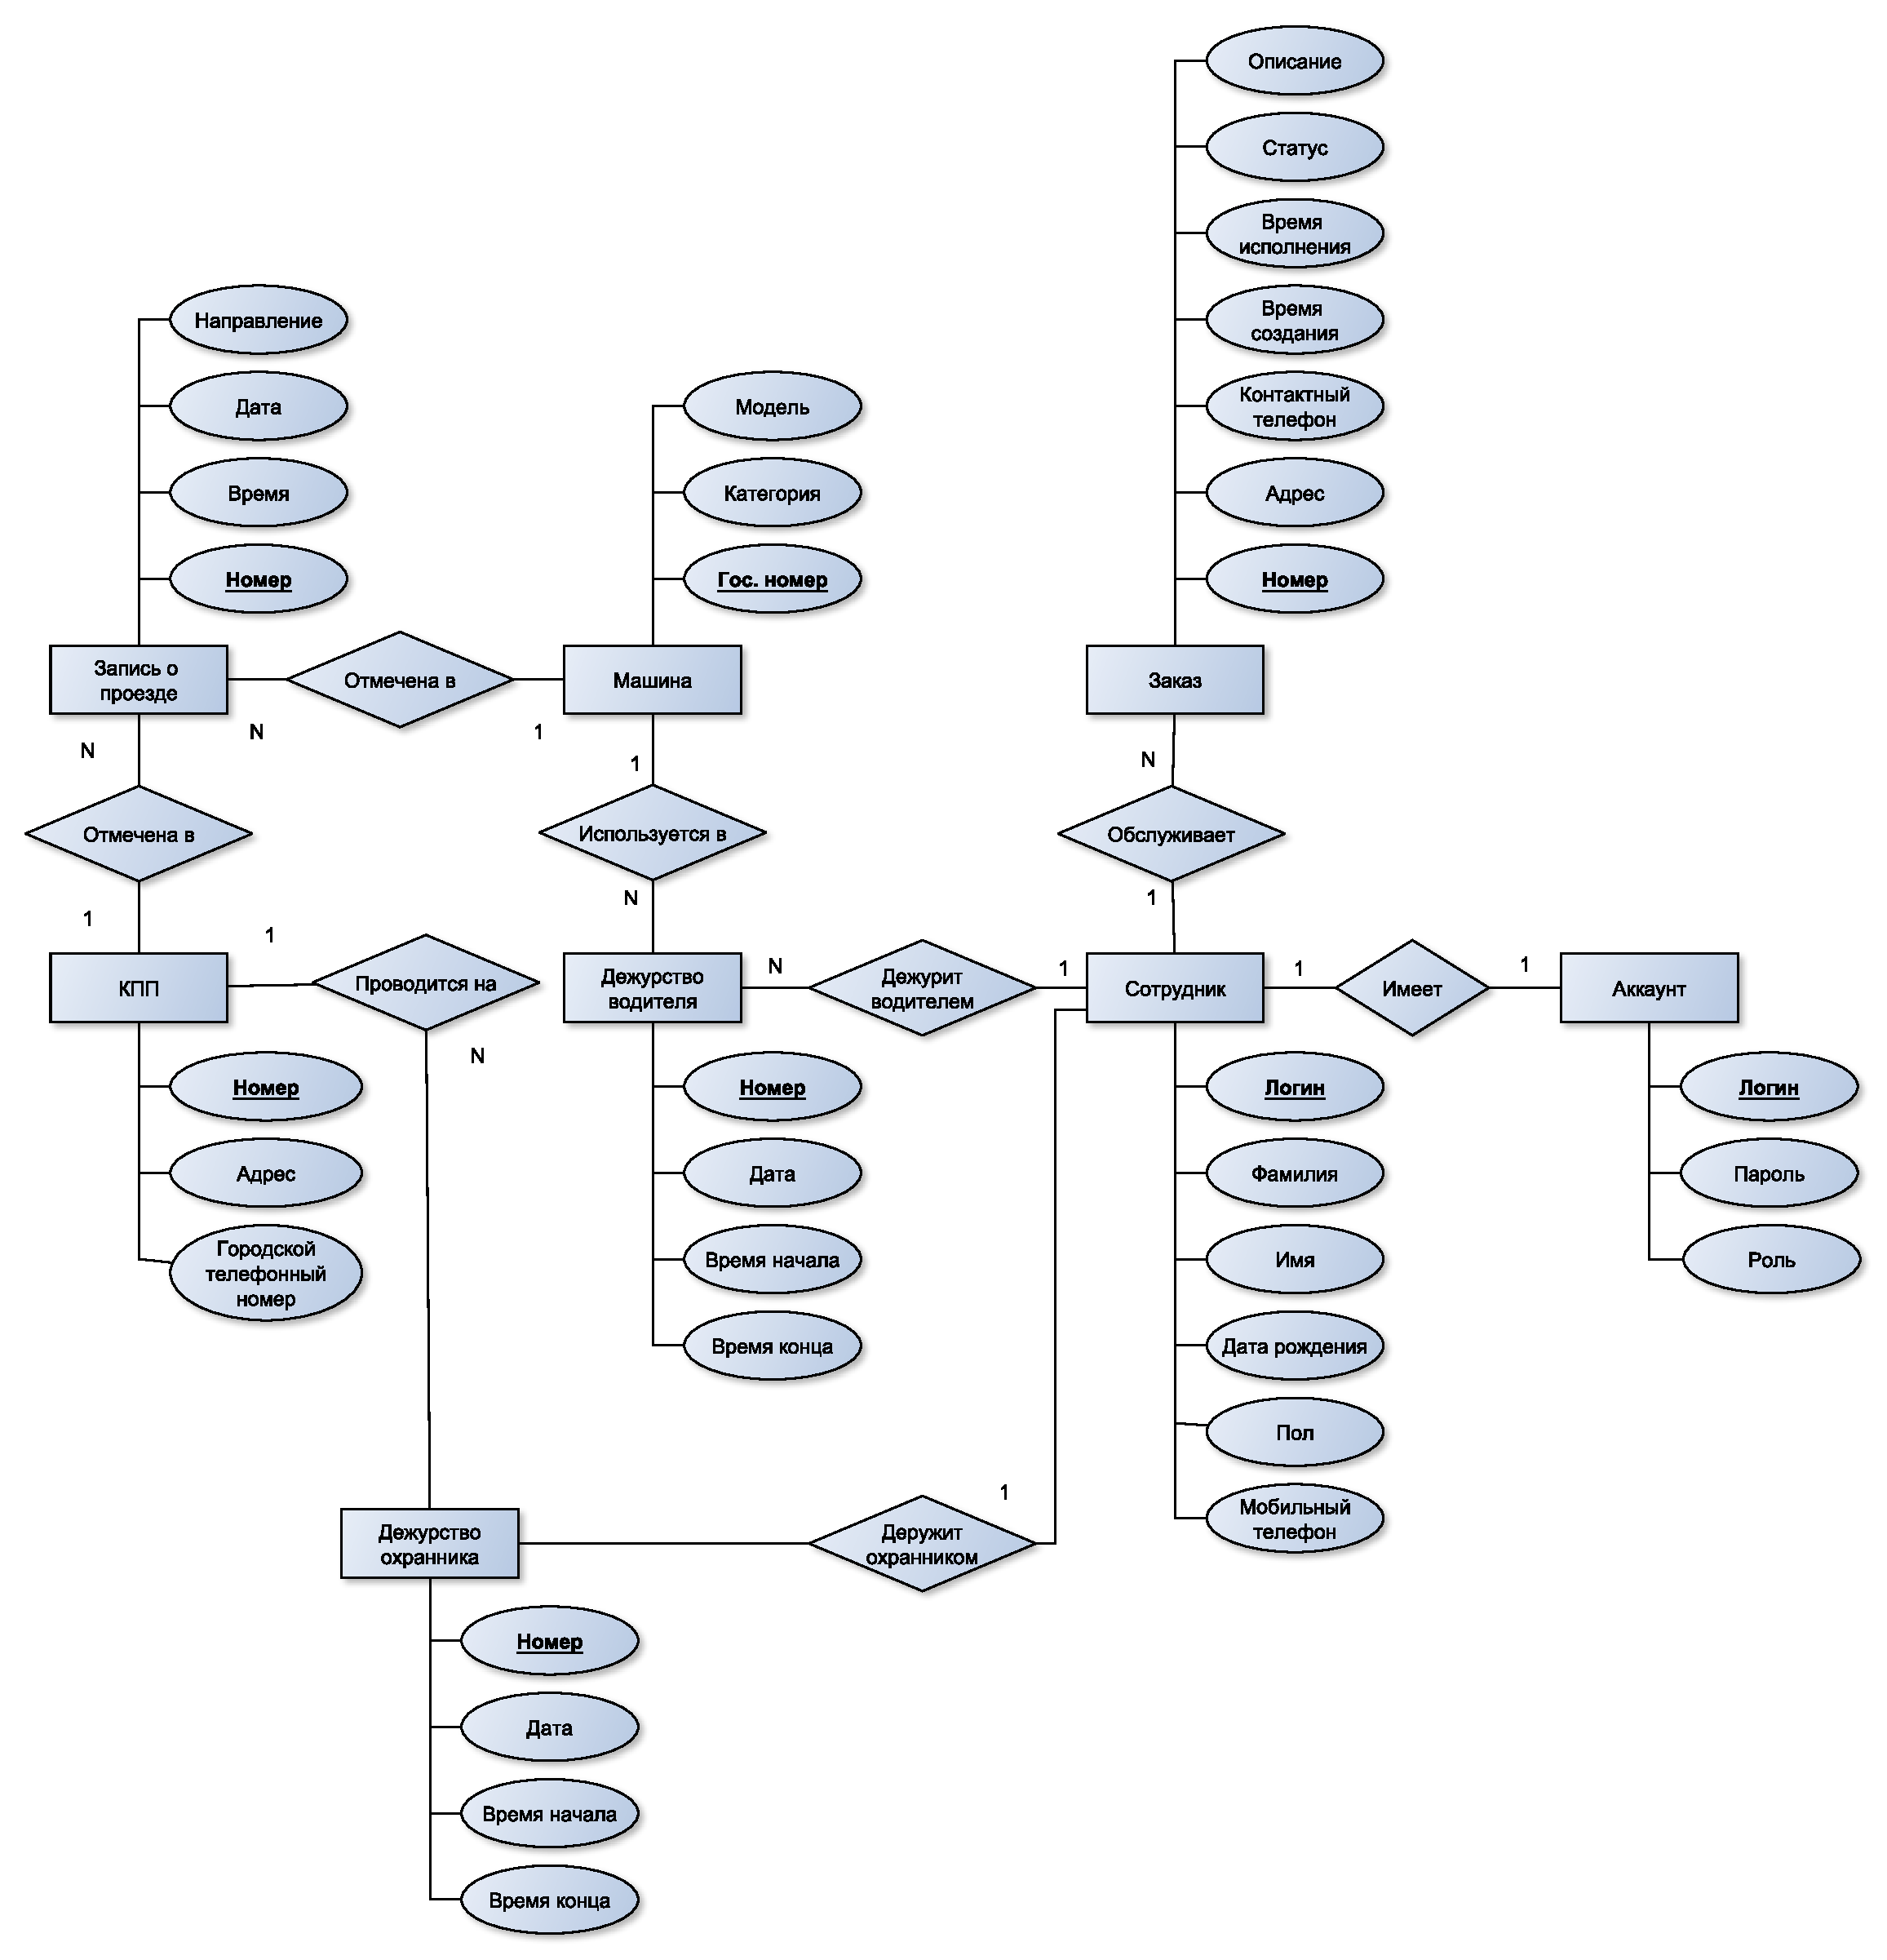
\includegraphics[height=18cm, width = 14cm]{schemes/er.pdf}}
		{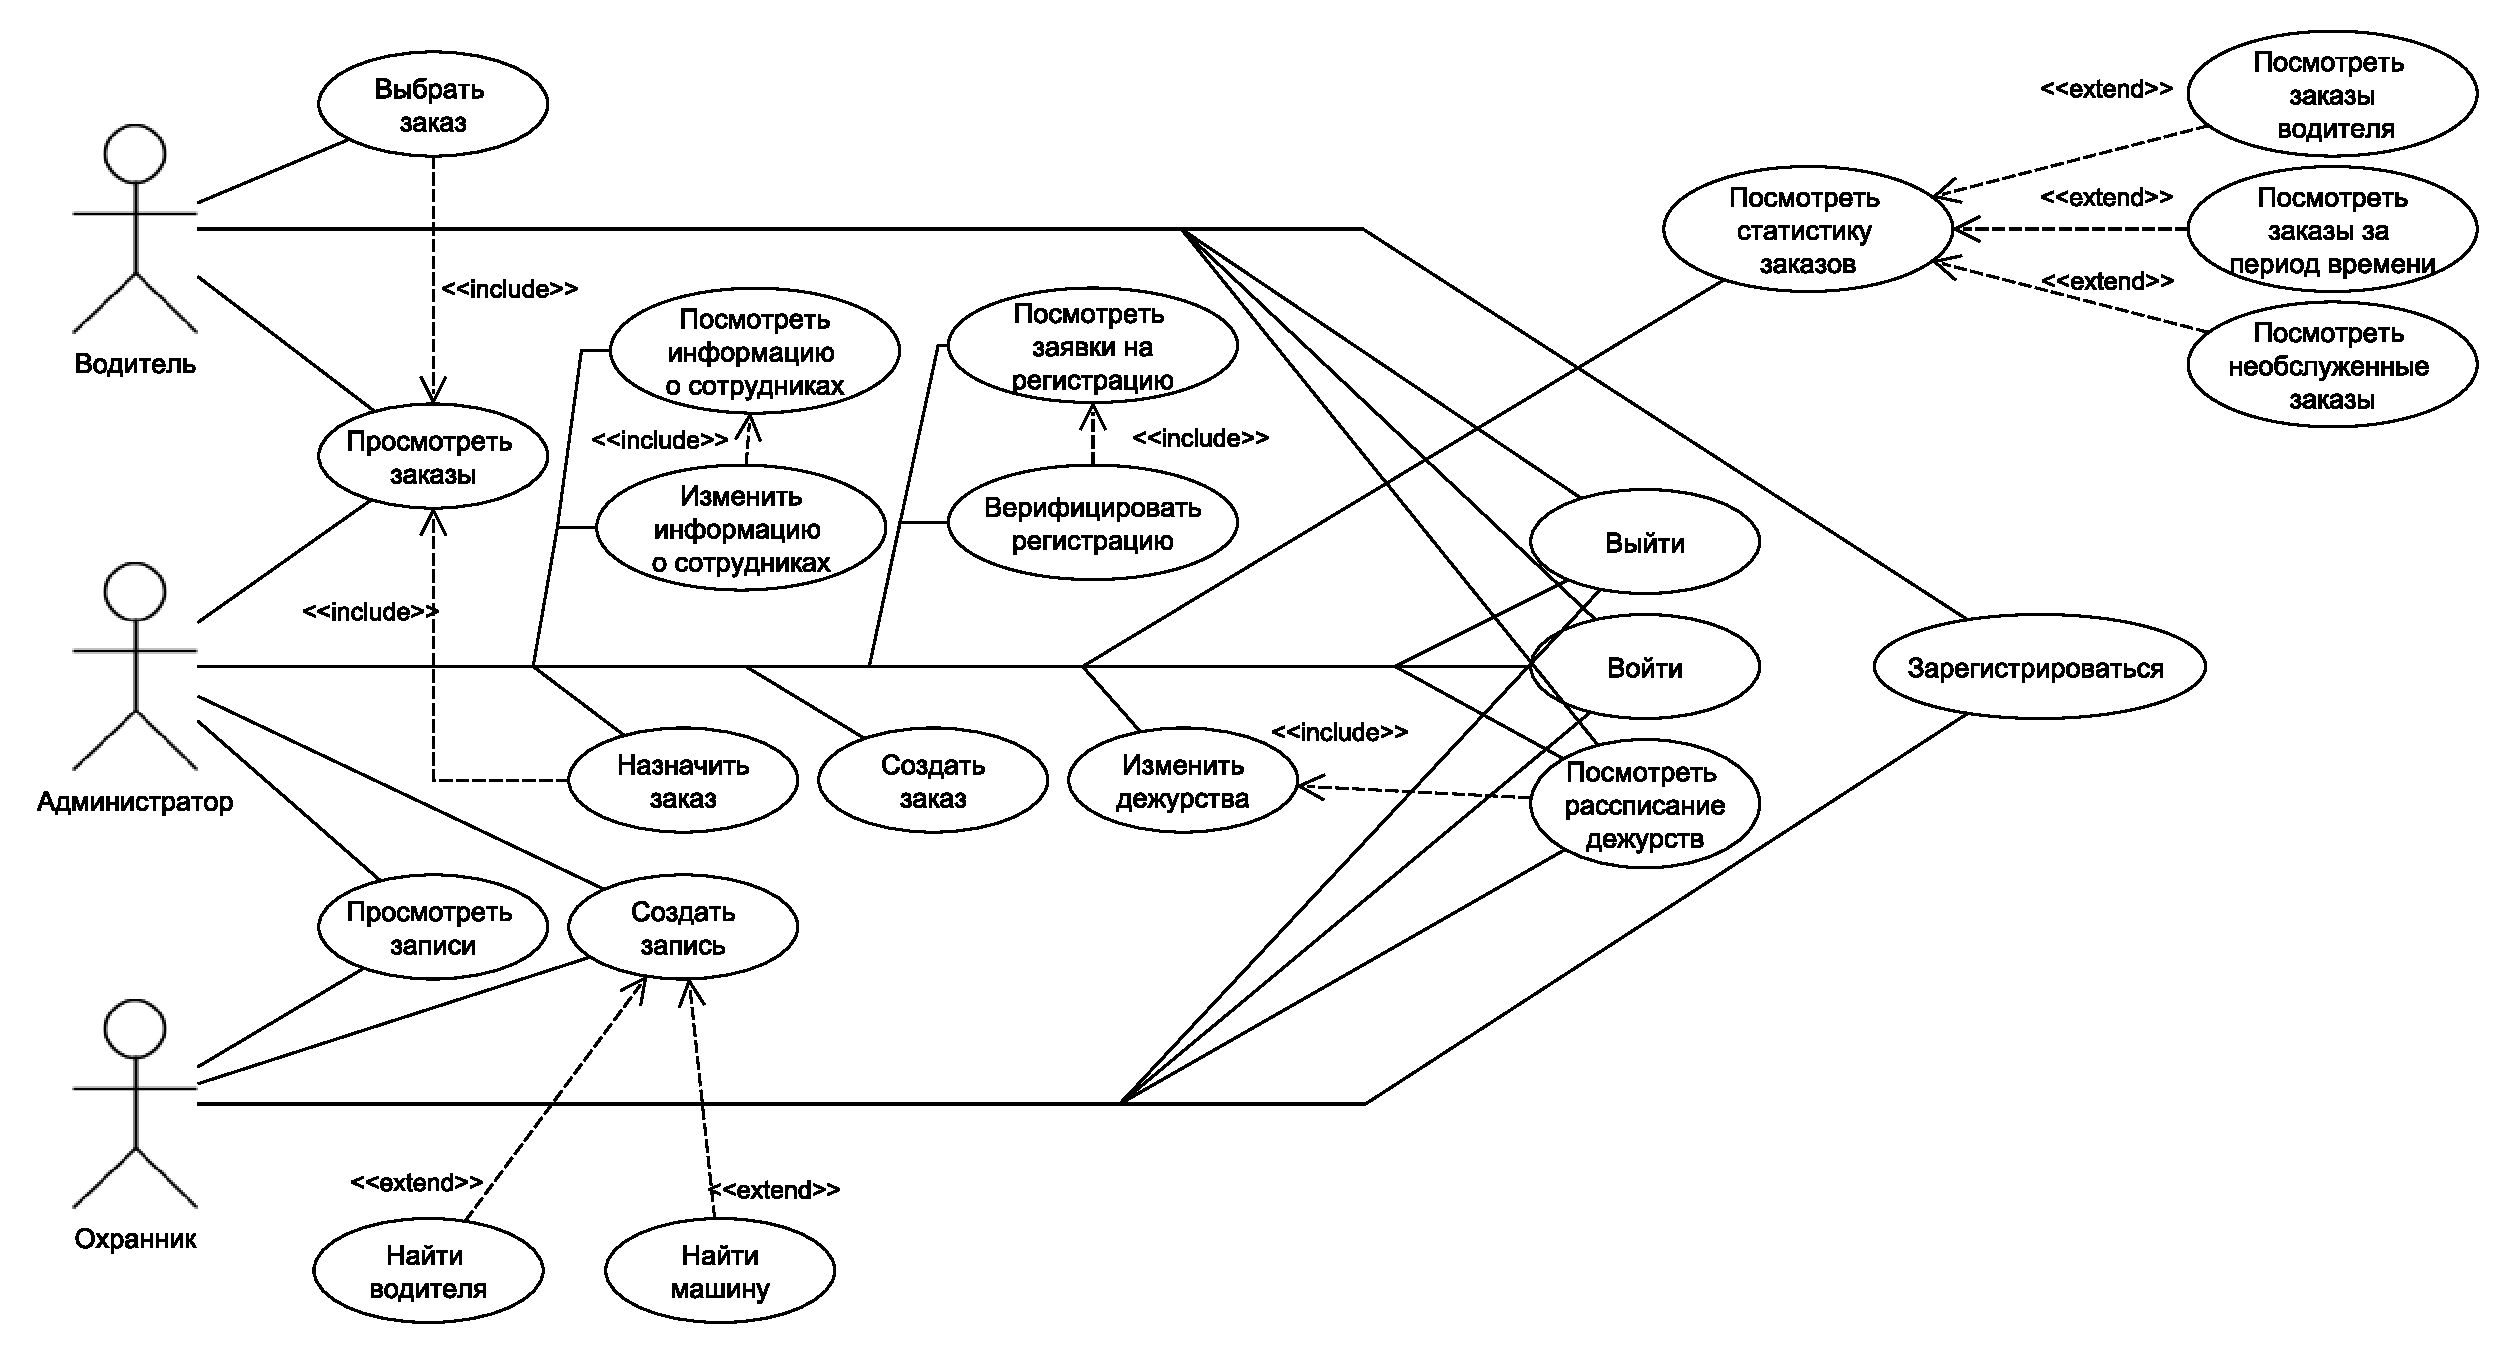
\includegraphics[scale=0.4, angle=-90]{schemes/use-case.pdf}}
		\caption{ER-диаграмма сущностей}
		\label{use_case}
	\end{center}
\end{figure}

\section{Проектирование базы данных}
\subsection{Сущности базы данных}
На рисунке \ref{er_db} представленна ER-диаграмма сущностей базы данных.

\begin{figure}[ph!]
	\begin{center}
		{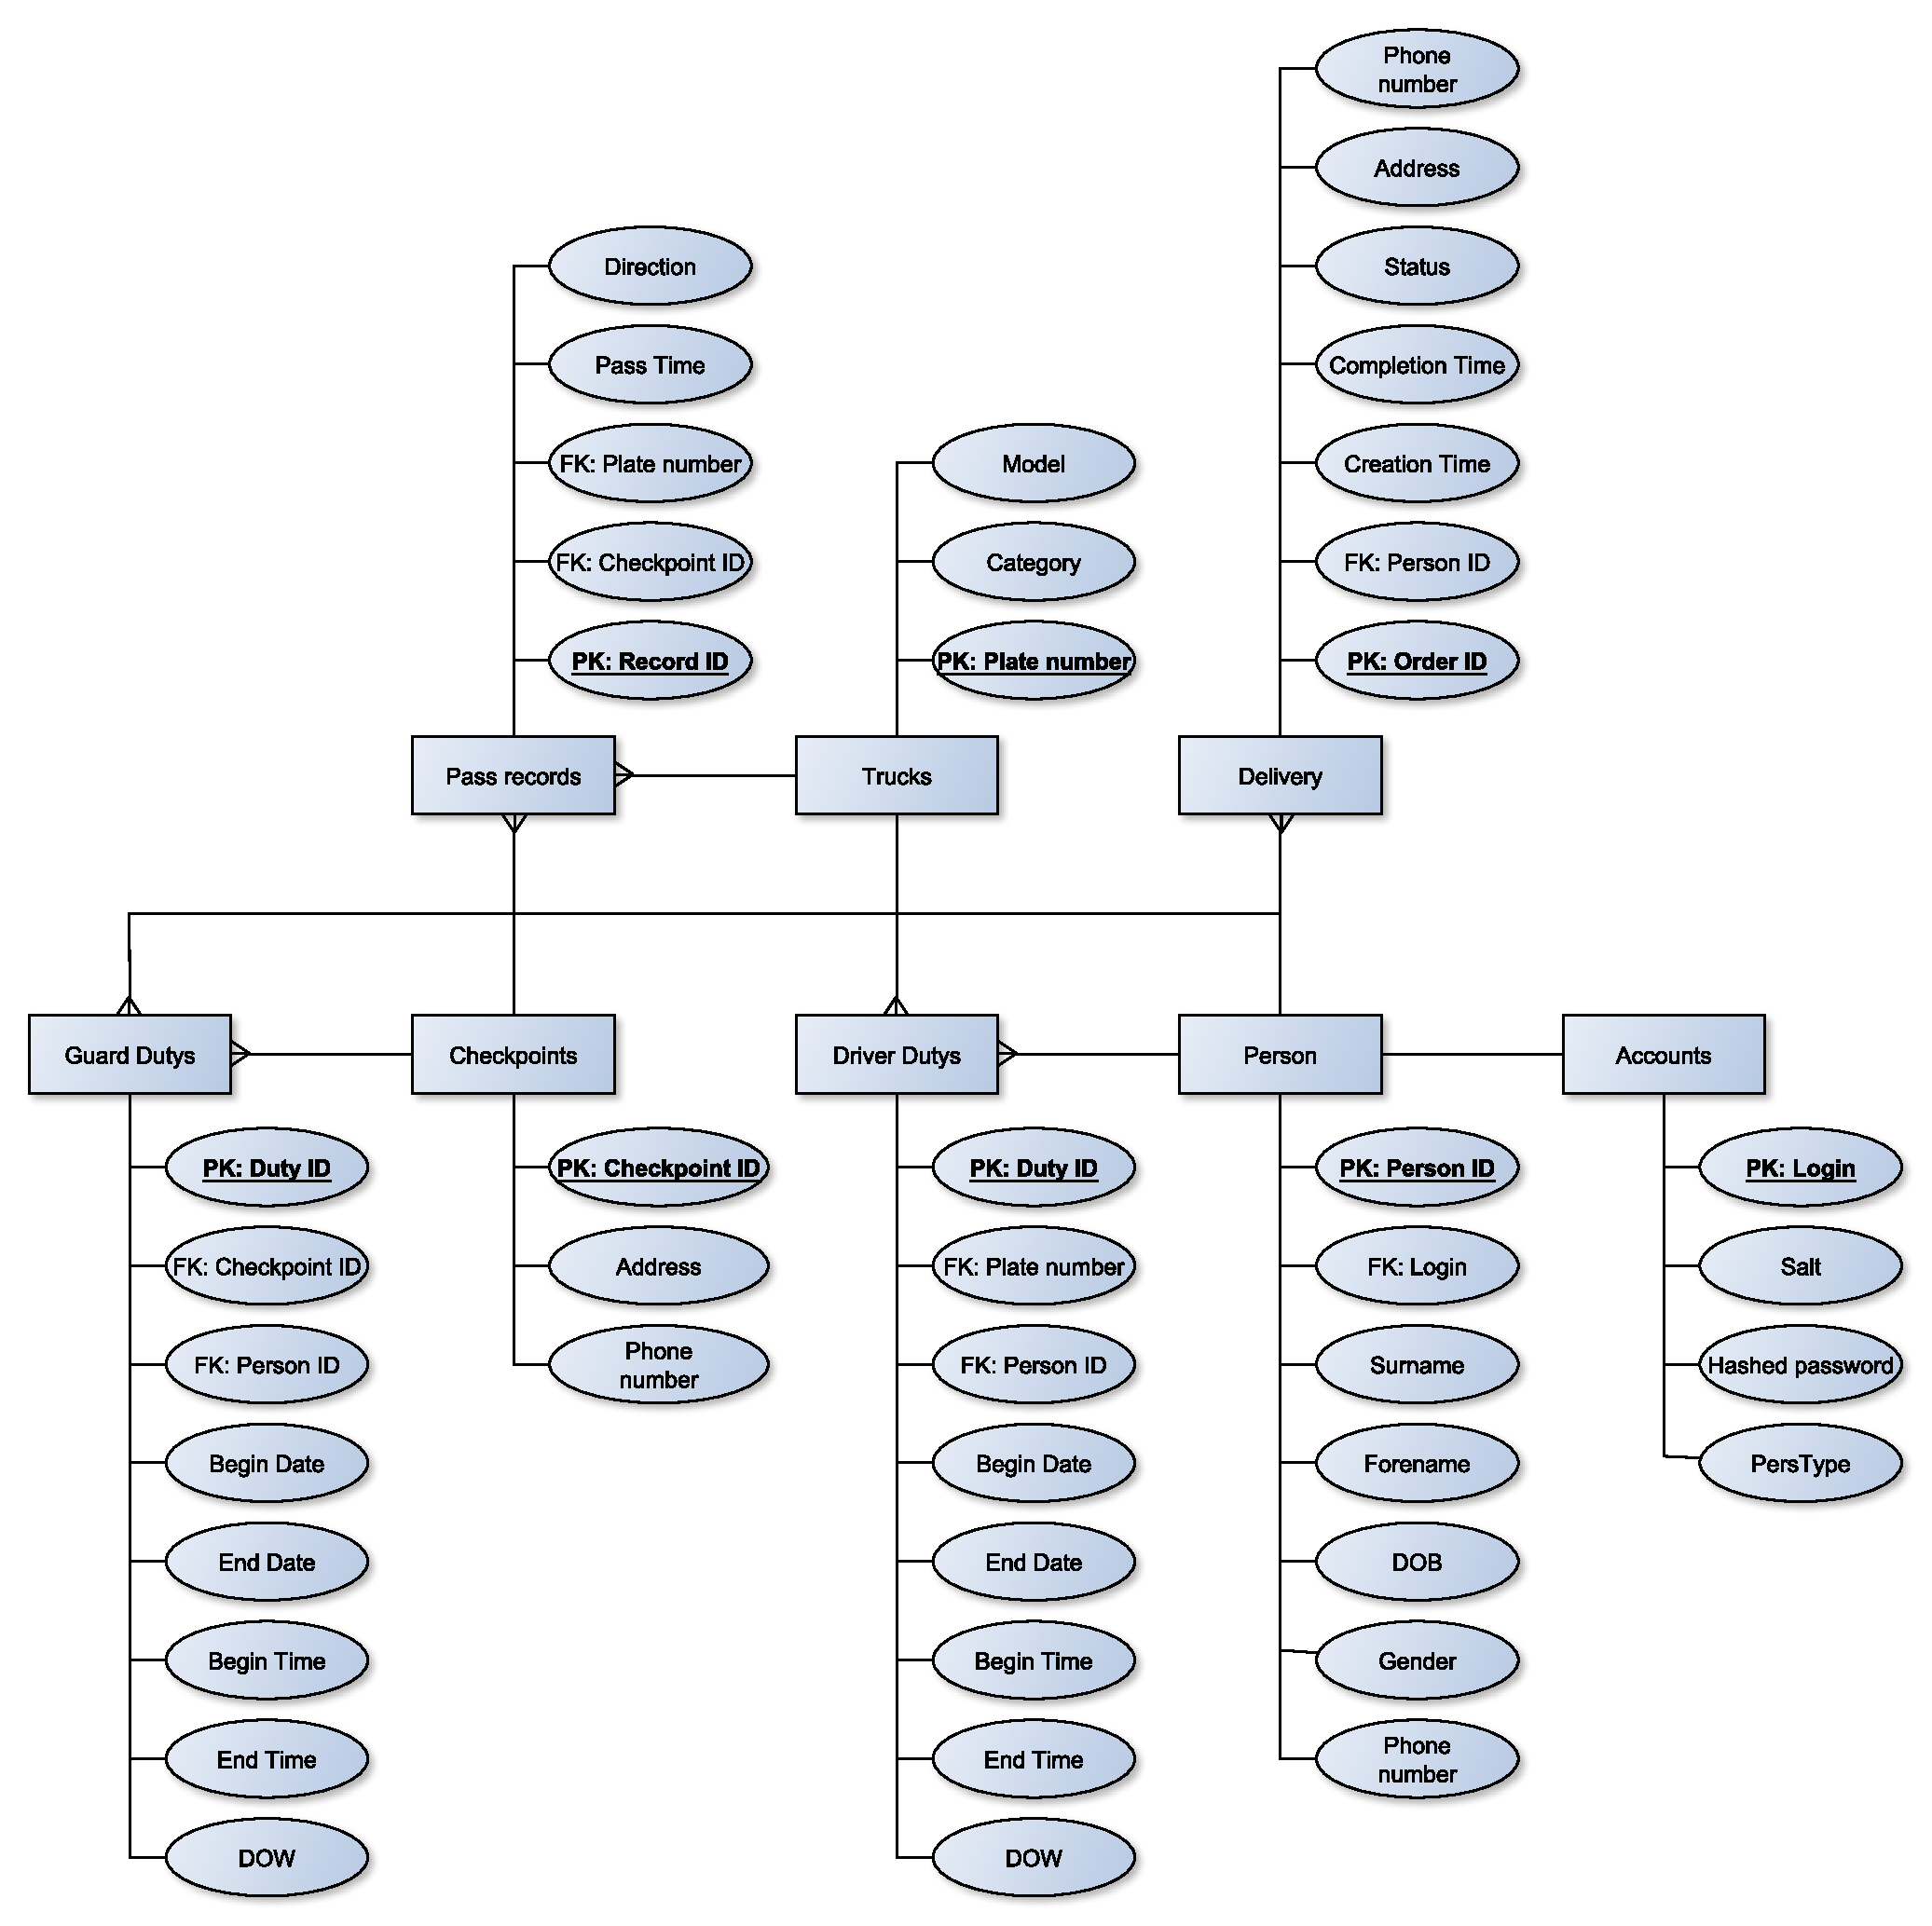
\includegraphics[height=14cm, width = 15cm]{schemes/er_db.pdf}}
%		{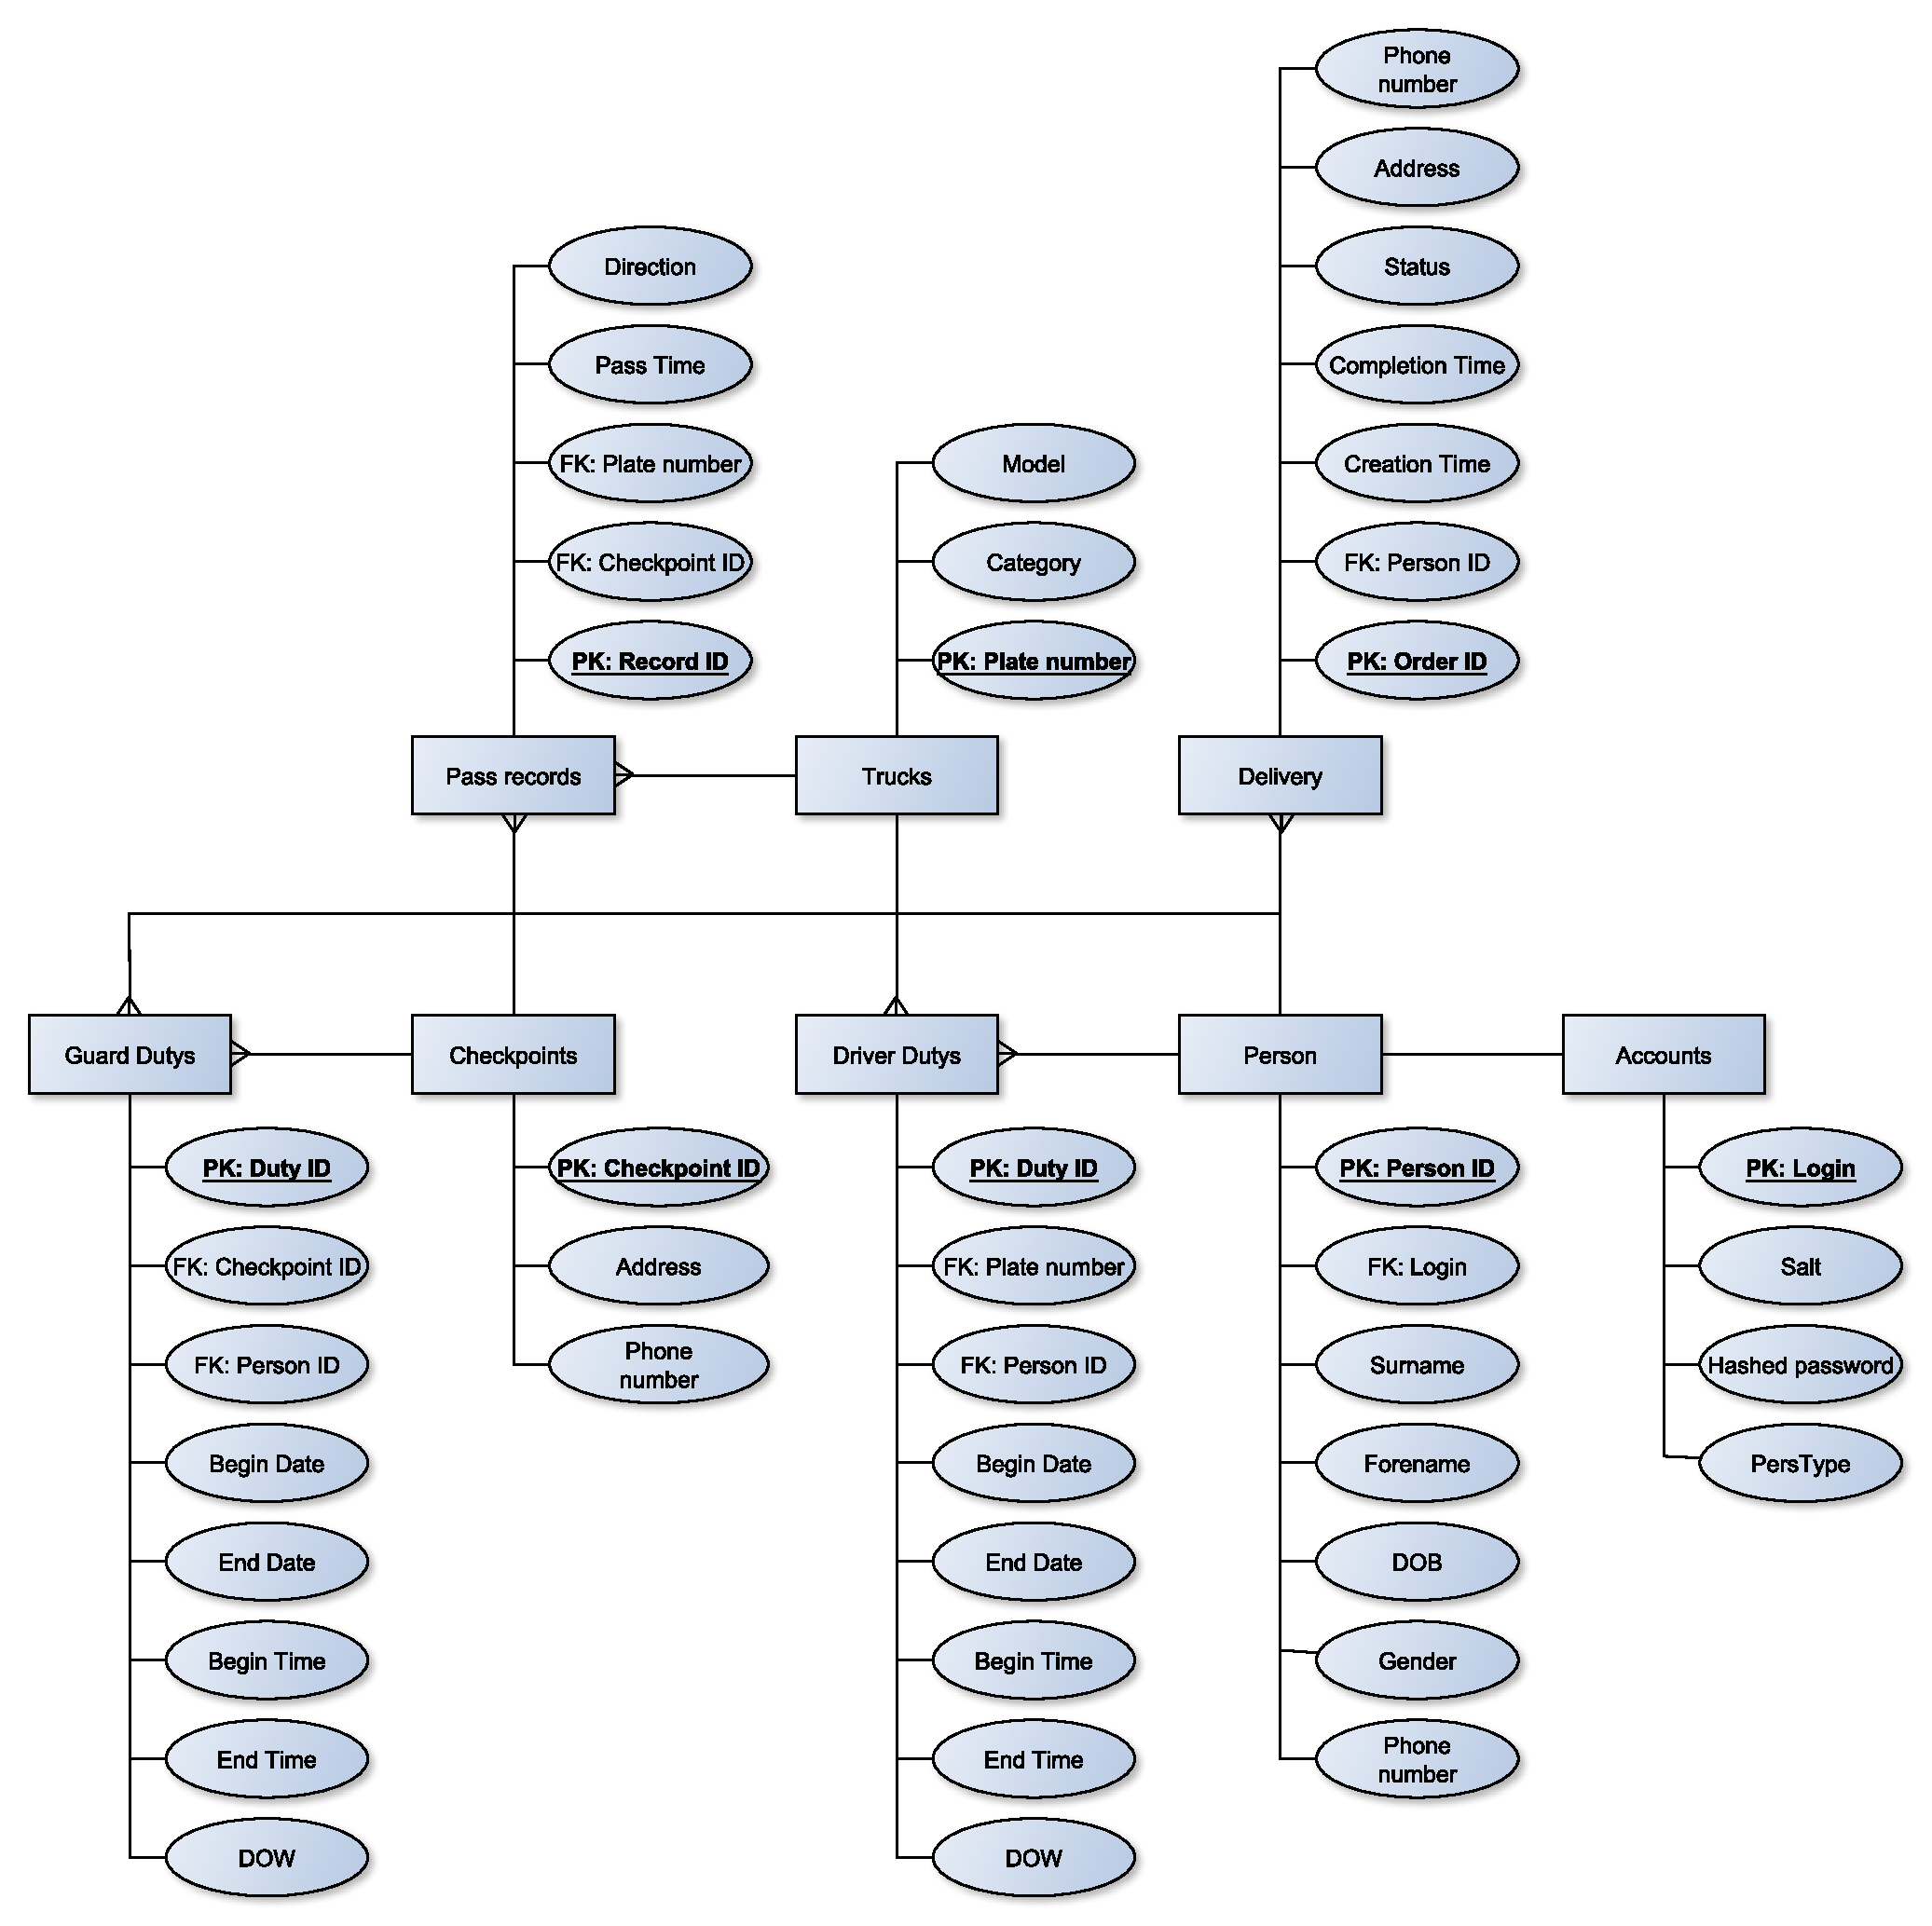
\includegraphics[scale=0.4, angle=0]{schemes/er_db.pdf}}
		\caption{ER-диаграмма сущностей базы данных}
		\label{er_db}
	\end{center}
\end{figure}

\subsection{Проектирование таблиц}
На основании выделенных сущностей база данных должна содержать таблицы, описание которых приведено в таблицах 2.1-2.8

Для обеспечения приватности пароля к аккаунту было принято решение использовать хэширование. В качестве ролей используются значения admin, driver, guard (соотв. администратор, водитель, охранник).
\begin{table}[h] 
	\begin{center}
	\caption{Accounts (таблица аккаунтов)}
	\label{acc_table}
	\begin{tabular}{| c | c | c |}
		\hline
		\textbf{Атрибут}		&	\textbf{Тип}		& \textbf{Комментарий} \\
		\hline
		Login 		&	Строка		&	Логин аккаунта, PK \\ \hline
		PersType 	&	Строка 		&	Роль аккаунта \\ \hline
		Salt 		&	Строка		&	"Соль" для хэширования пароля \\ \hline
		HashedPassword & Строка		&	Хэшированный пароль \\ \hline
	\end{tabular}
	\end{center}
\end{table}

\begin{table}[h] 
	\begin{center}
		\caption{Person (таблица личной информации)}
		\label{pers_table}
		\begin{tabular}{| c | c | c |}
			\hline
			\textbf{Атрибут}		&	\textbf{Тип}		& \textbf{Комментарий} \\
			\hline
			Login 		&	Строка		&	Логин аккаунта, PK, FK \\ \hline
			Surname 	&	Строка 		&	Фамилия сотрудника \\ \hline
			Forename 	&	Строка 		&	Имя сотрудника \\ \hline
			DOB 		&	Дата		&	Дата рождения сотрудника \\ \hline
			Gender 		&   Строка		&	Пол сотрудника \\ \hline
			PhoneNumber	&   Строка		&	Номер мобильного телефона сотрудника \\ \hline
		\end{tabular}
	\end{center}
\end{table}

\begin{table}[h!] 
	\begin{center}
		\caption{Trucks (таблица машин)}
		\label{truck_table}
		\begin{tabular}{| c | c | p{10cm} |}
			\hline
			\textbf{Атрибут}		&	\textbf{Тип}		& \textbf{Комментарий} \\
			\hline
			PlateNumber	&	Строка	&	Гос. номер машины, PK \\ \hline
			Category	&	Строка	&	Марка машины \\ \hline
			Model		&	Строка	&	Модель машины \\ \hline
		\end{tabular}
	\end{center}
\end{table}

В качестве статуса заказа используются значения not\_assigned, in\_transit, delivered (соотв. заказ не назначен водителю, заказ в процессе доставки и заказ доставлен).
\begin{table}[h!] 
	\begin{center}
		\caption{Delivery (таблица заказов)}
		\label{del_table}
		\begin{tabular}{| c | c | p{8cm} |}
			\hline
			\textbf{Атрибут}		&	\textbf{Тип}		& \textbf{Комментарий} \\
			\hline
			OrderID		&	Целое число	&	Уникальный номер заказа, PK \\ \hline
			Login 		&	Строка		&	Логин водителя, доставляющего или доставившего заказ, FK \\ \hline
			Address 	&	Строка 		&	Адрес заказчика \\ \hline
			PhoneNumber	&	Строка 		&	Контакты заказчика \\ \hline
			Status 		& 	Строка		&	Статус заказа \\ \hline
			Description	& 	Строка		&	Содержание заказа \\ \hline
			CreationTime	& Дата, время	&	Дата и время создания заказа \\ \hline
			CompletionTime	& Дата, время	&	Дата и время завершения заказа \\ \hline
		\end{tabular}
	\end{center}
\end{table}

\begin{table}[h!] 
	\begin{center}
		\caption{Checkpoints (таблица КПП)}
		\label{checkp_table}
		\begin{tabular}{| c | c | c |}
			\hline
			\textbf{Атрибут}		&	\textbf{Тип}		& \textbf{Комментарий} \\
			\hline
			CheckpointID	&	Целое число	&	Номер КПП, PK \\ \hline
			Address			&	Строка		&	Адрес КПП \\ \hline
			PhoneNumber		&	Строка		&	Номер телефона КПП \\ \hline
		\end{tabular}
	\end{center}
\end{table}


Дежурства как охранников, так и водителей имеют цикличный характер по неделе. Поэтому рациональнее хранить не каждое дежурство отдельно, а правило, содержащее диапазон дат и дни недели, в которые сотрудник дежурит. Атрибут дней недели в таблице хранит строку, определяющую дни по номеру (например строка 013 соответсвует дежурству по понедельникам, вторникам и четвергам). Период (или расписание) дежурства выделено в отдельную таблицу.

\begin{table}[h!]
	\begin{center}
		\caption{DutyRules (таблица расписаний дежурств)}
		\label{dutyrule_table}
		\begin{tabular}{| c | c | p{8cm} |}
			\hline
			\textbf{Атрибут}		&	\textbf{Тип}		& \textbf{Комментарий} \\
			\hline
			RuleID		&	Целое число	&	Номер периода дежурства, PK \\ \hline
			BeginDate 	&	Дата		&	Дата начала периода дежурства \\ \hline
			EndDate 	&	Дата		&	Дата окончания периода дежурства \\ \hline
			BeginTime 	&	Время		&	Время начала дежурства \\ \hline
			EndTime 	&	Время		&	Время окончания дежурства \\ \hline
			DOW 		&	Строка		&	Дни недели дежурства \\ \hline
		\end{tabular}
	\end{center}
\end{table}

\begin{table}[h!]
	\begin{center}
		\caption{GuardDutys (таблица дежурств охранников)}
		\label{gduty_table}
		\begin{tabular}{| c | c | p{8cm} |}
			\hline
			\textbf{Атрибут}		&	\textbf{Тип}		& \textbf{Комментарий} \\
			\hline
			DutyID		&	Целое число	&	Номер дежурства, PK \\ \hline
			Login 		&	Строка		&	Логин дежурящего охранника, FK \\ \hline
			CheckpointID &	Целое число	&	Номер КПП, FK \\ \hline
			RuleID		&	Целое число	&	Номер периода дежурства, FK \\ \hline
		\end{tabular}
	\end{center}
\end{table}

\begin{table}[h!] 
	\begin{center}
		\caption{DriverDutys (таблица дежурств водителей)}
		\label{dduty_table}
		\begin{tabular}{| c | c | p{8cm} |}
			\hline
			\textbf{Атрибут}		&	\textbf{Тип}		& \textbf{Комментарий} \\
			\hline
			DutyID		&	Целое число	&	Номер дежурства, PK \\ \hline
			Login 		&	Строка		&	Логин дежурящего водителя, FK \\ \hline
			PlateNumber &	Строка		&	Гос. номер машины, FK \\ \hline
			RuleID		&	Целое число	&	Номер периода дежурства, FK \\ \hline
		\end{tabular}
	\end{center}
\end{table}

В качестве направления проезда используются значения in, out (соотв. въезд и выезд с территории предприятия).
\newpage
\begin{table}[h!] 
	\begin{center}
		\caption{PassRecords (таблица записей проездов)}
		\label{pass_table}
		\begin{tabular}{| c | c | c |}
			\hline
			\textbf{Атрибут}		&	\textbf{Тип}		& \textbf{Комментарий} \\
			\hline
			RecordID	&	Целое число	&	Номер записи, PK \\ \hline
			PlateNumber	&	Строка		&	Гос. номер машины, FK \\ \hline
			CheckpointID &	Целое число	&	Номер КПП, FK \\ \hline
			PassTime 	&	Дата, время	&	Дата и время проезда \\ \hline
			Direction 	&	Строка		&	Направление проезда \\ \hline
		\end{tabular}
	\end{center}
\end{table}

Также было принято создать таблицу для хранения информации о событиях в базе данных.
\begin{table}[h!] 
	\begin{center}
		\caption{LogActions (таблица активности пользователей)}
		\label{pass_table}
		\begin{tabular}{| c | c | c |}
			\hline
			\textbf{Атрибут}		&	\textbf{Тип}		& \textbf{Комментарий} \\
			\hline
			Actor	&	Строка	&	Роль, осуществившая действие \\ \hline
			ActTime	&	Дата, время		&	Время действия \\ \hline
			Description &	Строка	&	Описание действия \\ \hline
		\end{tabular}
	\end{center}
\end{table}

\subsection{Нормализация схем отношений}
Распространённым подходом в проектировании баз данных является метод нормализации, служащий для устранения избыточности и упрощения контроля целостности. При проектировании данной базы данных была поставленна цель соответствия третьей нормальной форме, что является достаточным для выполнения описанных целей нормализации\cite{norm_db}.

В разработанной модели данных переменная отношения находитя в первой нормальной форме, так как выполняется условие атомарности. В каждом кортеже, соответствующем некоторой описанной таблице, каждый компонент является атомарным, то есть содержит только одно значение для каждого из атрибутов\cite{norm_db2}. Данное утверждение основанно на том, что каждый атрибут имеет простой тип данных.

Также созданная переменная отношения находится во второй нормальной форме, так как в каждой таблице любой не ключевой атрибут полностью зависит от первичного ключа. Для перехода в данную форму из таблиц дежурств охранников и водителей была отдельно выделена таблица расписаний дежурств.

Можно утверждать, что спроектированная переменная отношения находится в третьей нормальной форме. Во всех таблицах не ключевые атрибуты не связаны отношениями между собой, поэтому можно утверждать, что они зависят от первичного ключа нетранзитивно, что и является условием нахождения в третьей нормальной форме.

\subsection{Схемы триггеров}
В соответствии с описанной ранее схемой взаимодействия, существуют некоторые действия, которые могут выполнять сразу несколько ролей. Для сбора дополнительной информации о данных действиях требуется реализовать следующие триггеры. \\



\begin{itemize}
	\item Триггер сохранения информации добавления записи о проезде. Данное действие может осуществлять как охранник, так и администратор, но таблица PassRecords не хранит информации об авторе, поэтому было решено создать данный триггер. Его схема представлена на рисунке \ref{pass_trig}
	
	\begin{figure}[h!]
		\begin{center}
%			{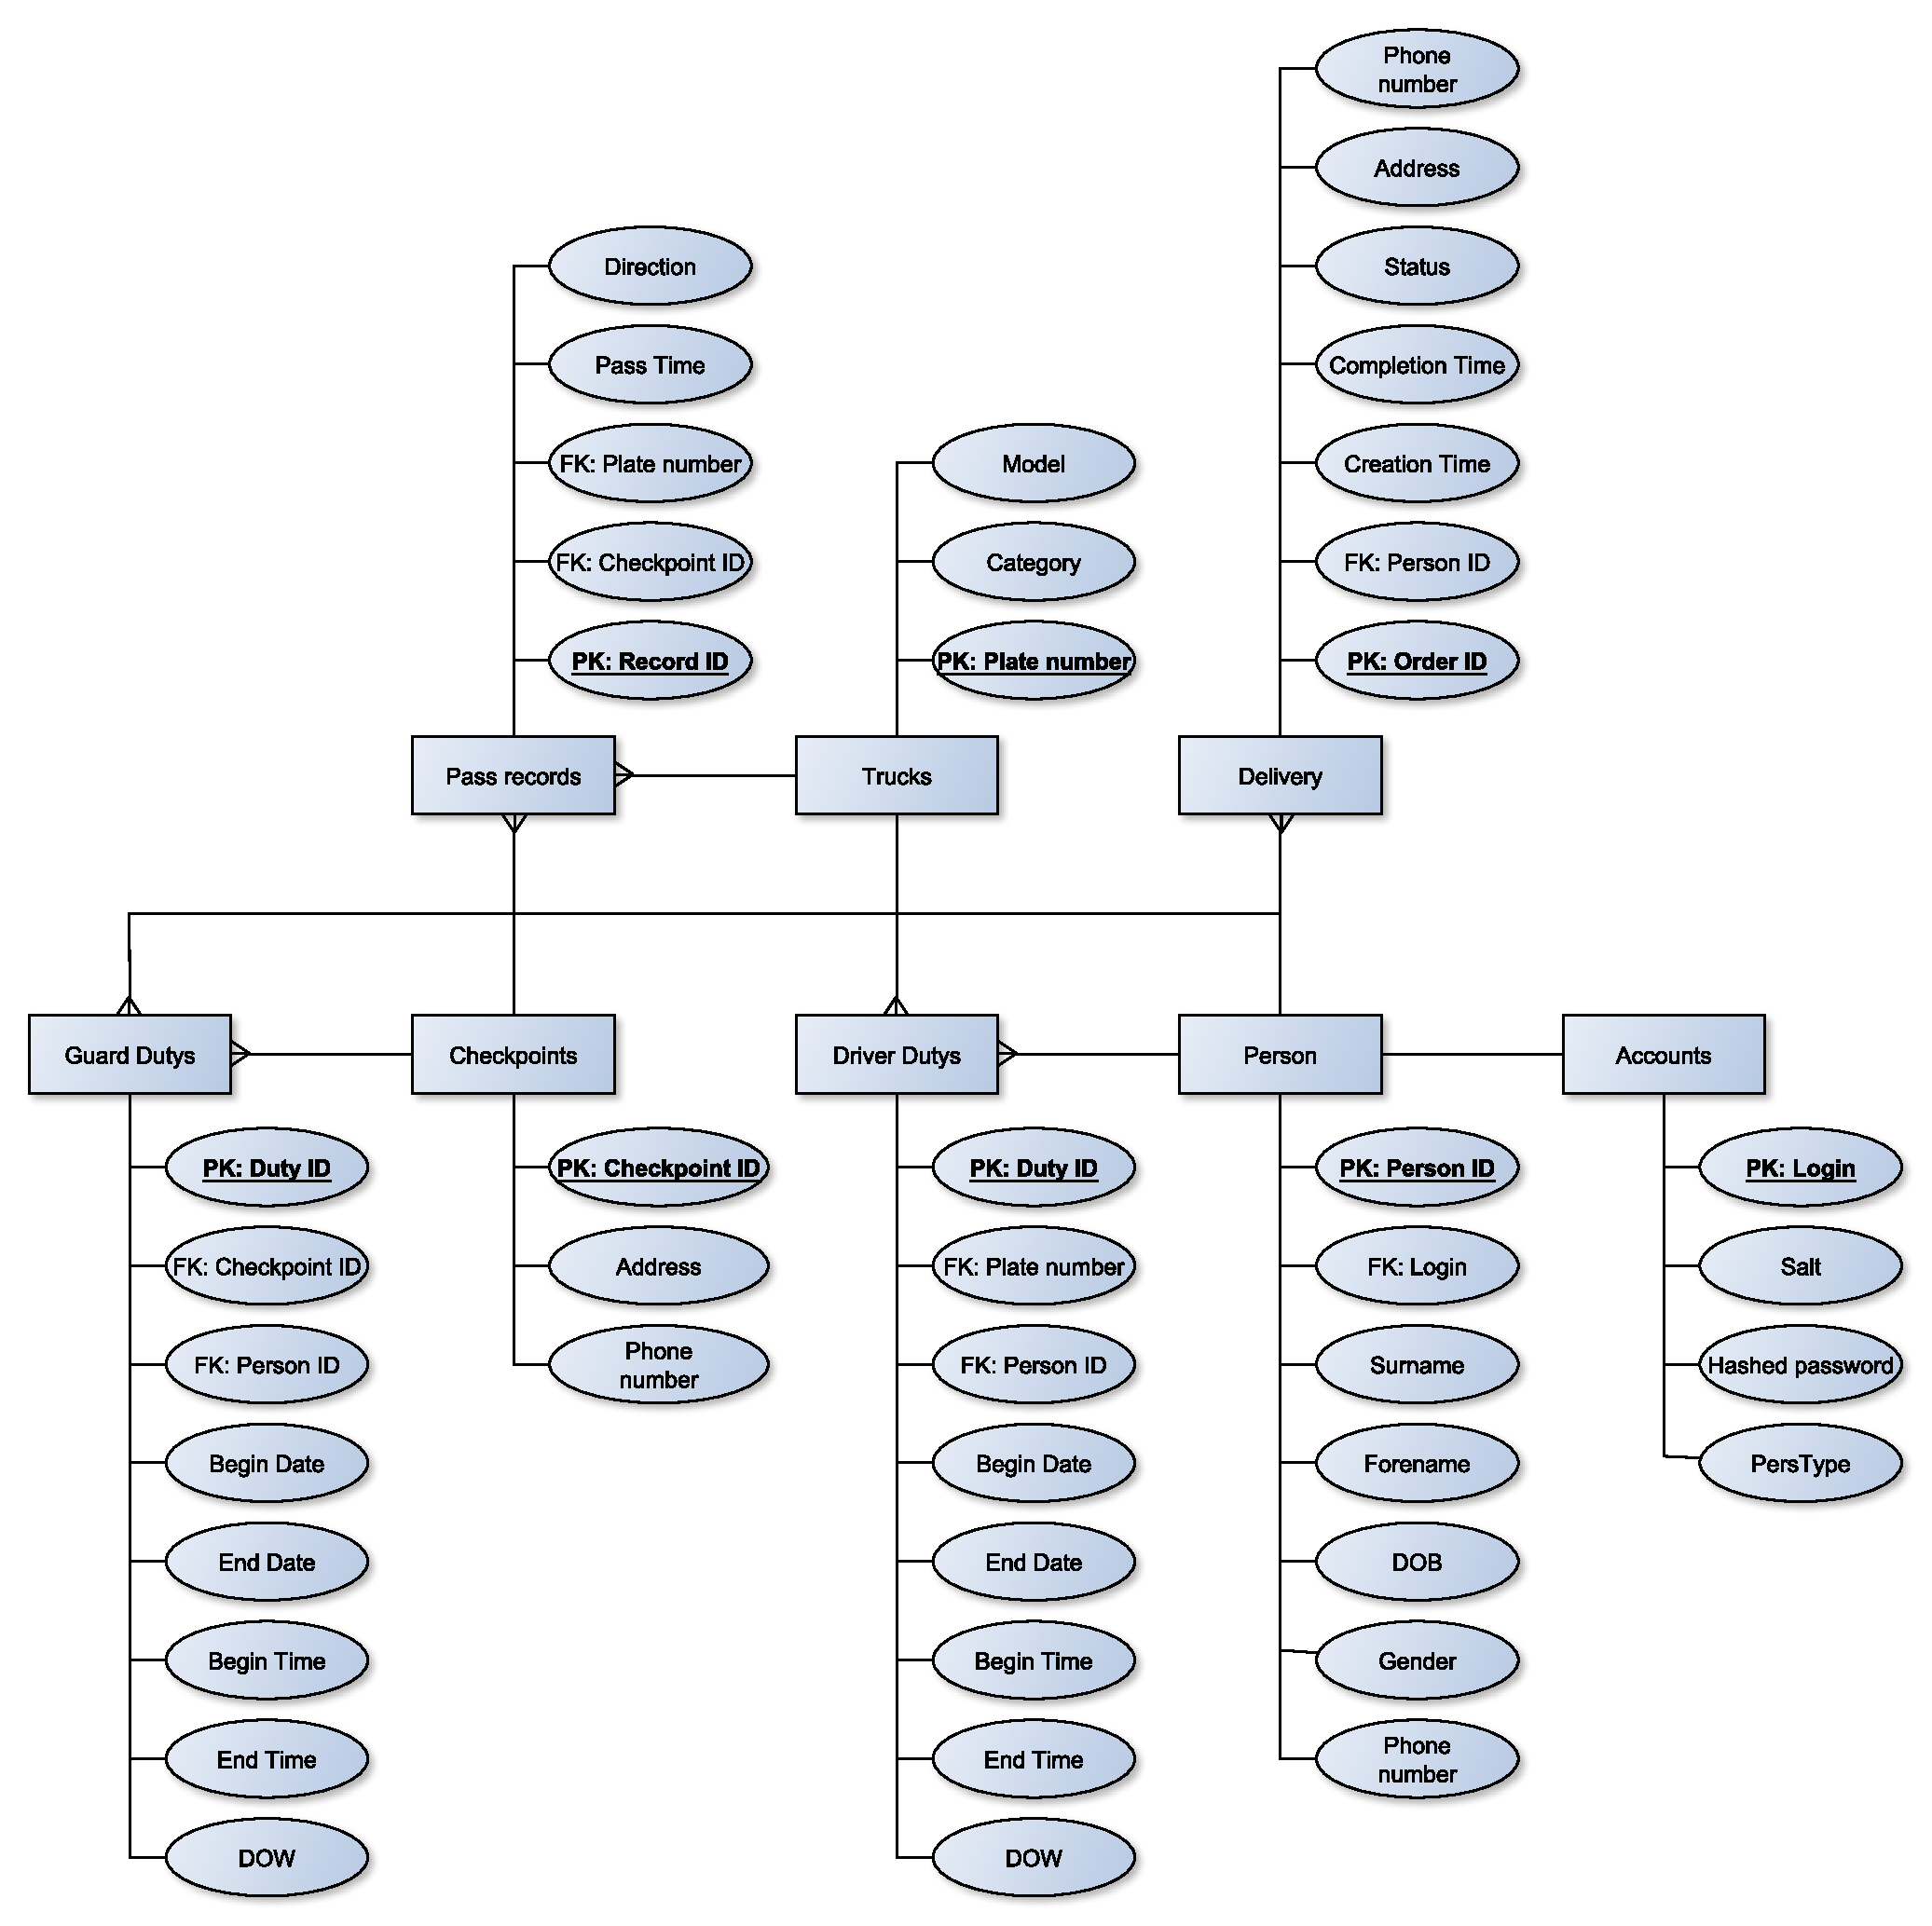
\includegraphics[height=14cm, width = 15cm]{schemes/er_db.pdf}}
			{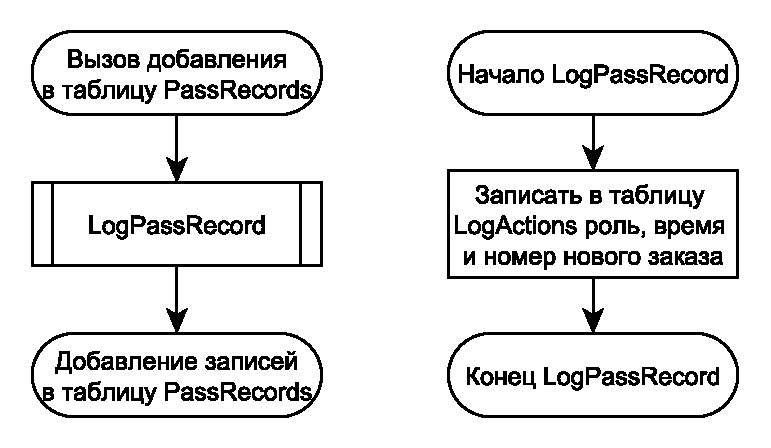
\includegraphics[scale=0.4, angle=0]{sql_schemes/pass_rec}}
			\caption{Схема алгоритма триггера на добавление в таблицу PassRecords}
			\label{pass_trig}
		\end{center}
	\end{figure}

	\item Триггер сохранения информации обновления заказа. В данном случае действие могут совершать водитель и администратор путём изменения статуса заказа и установлением времени его доставки. Его схема представлена на рисунке \ref{del_trig}
	
	\begin{figure}[h!]
		\begin{center}
			%			{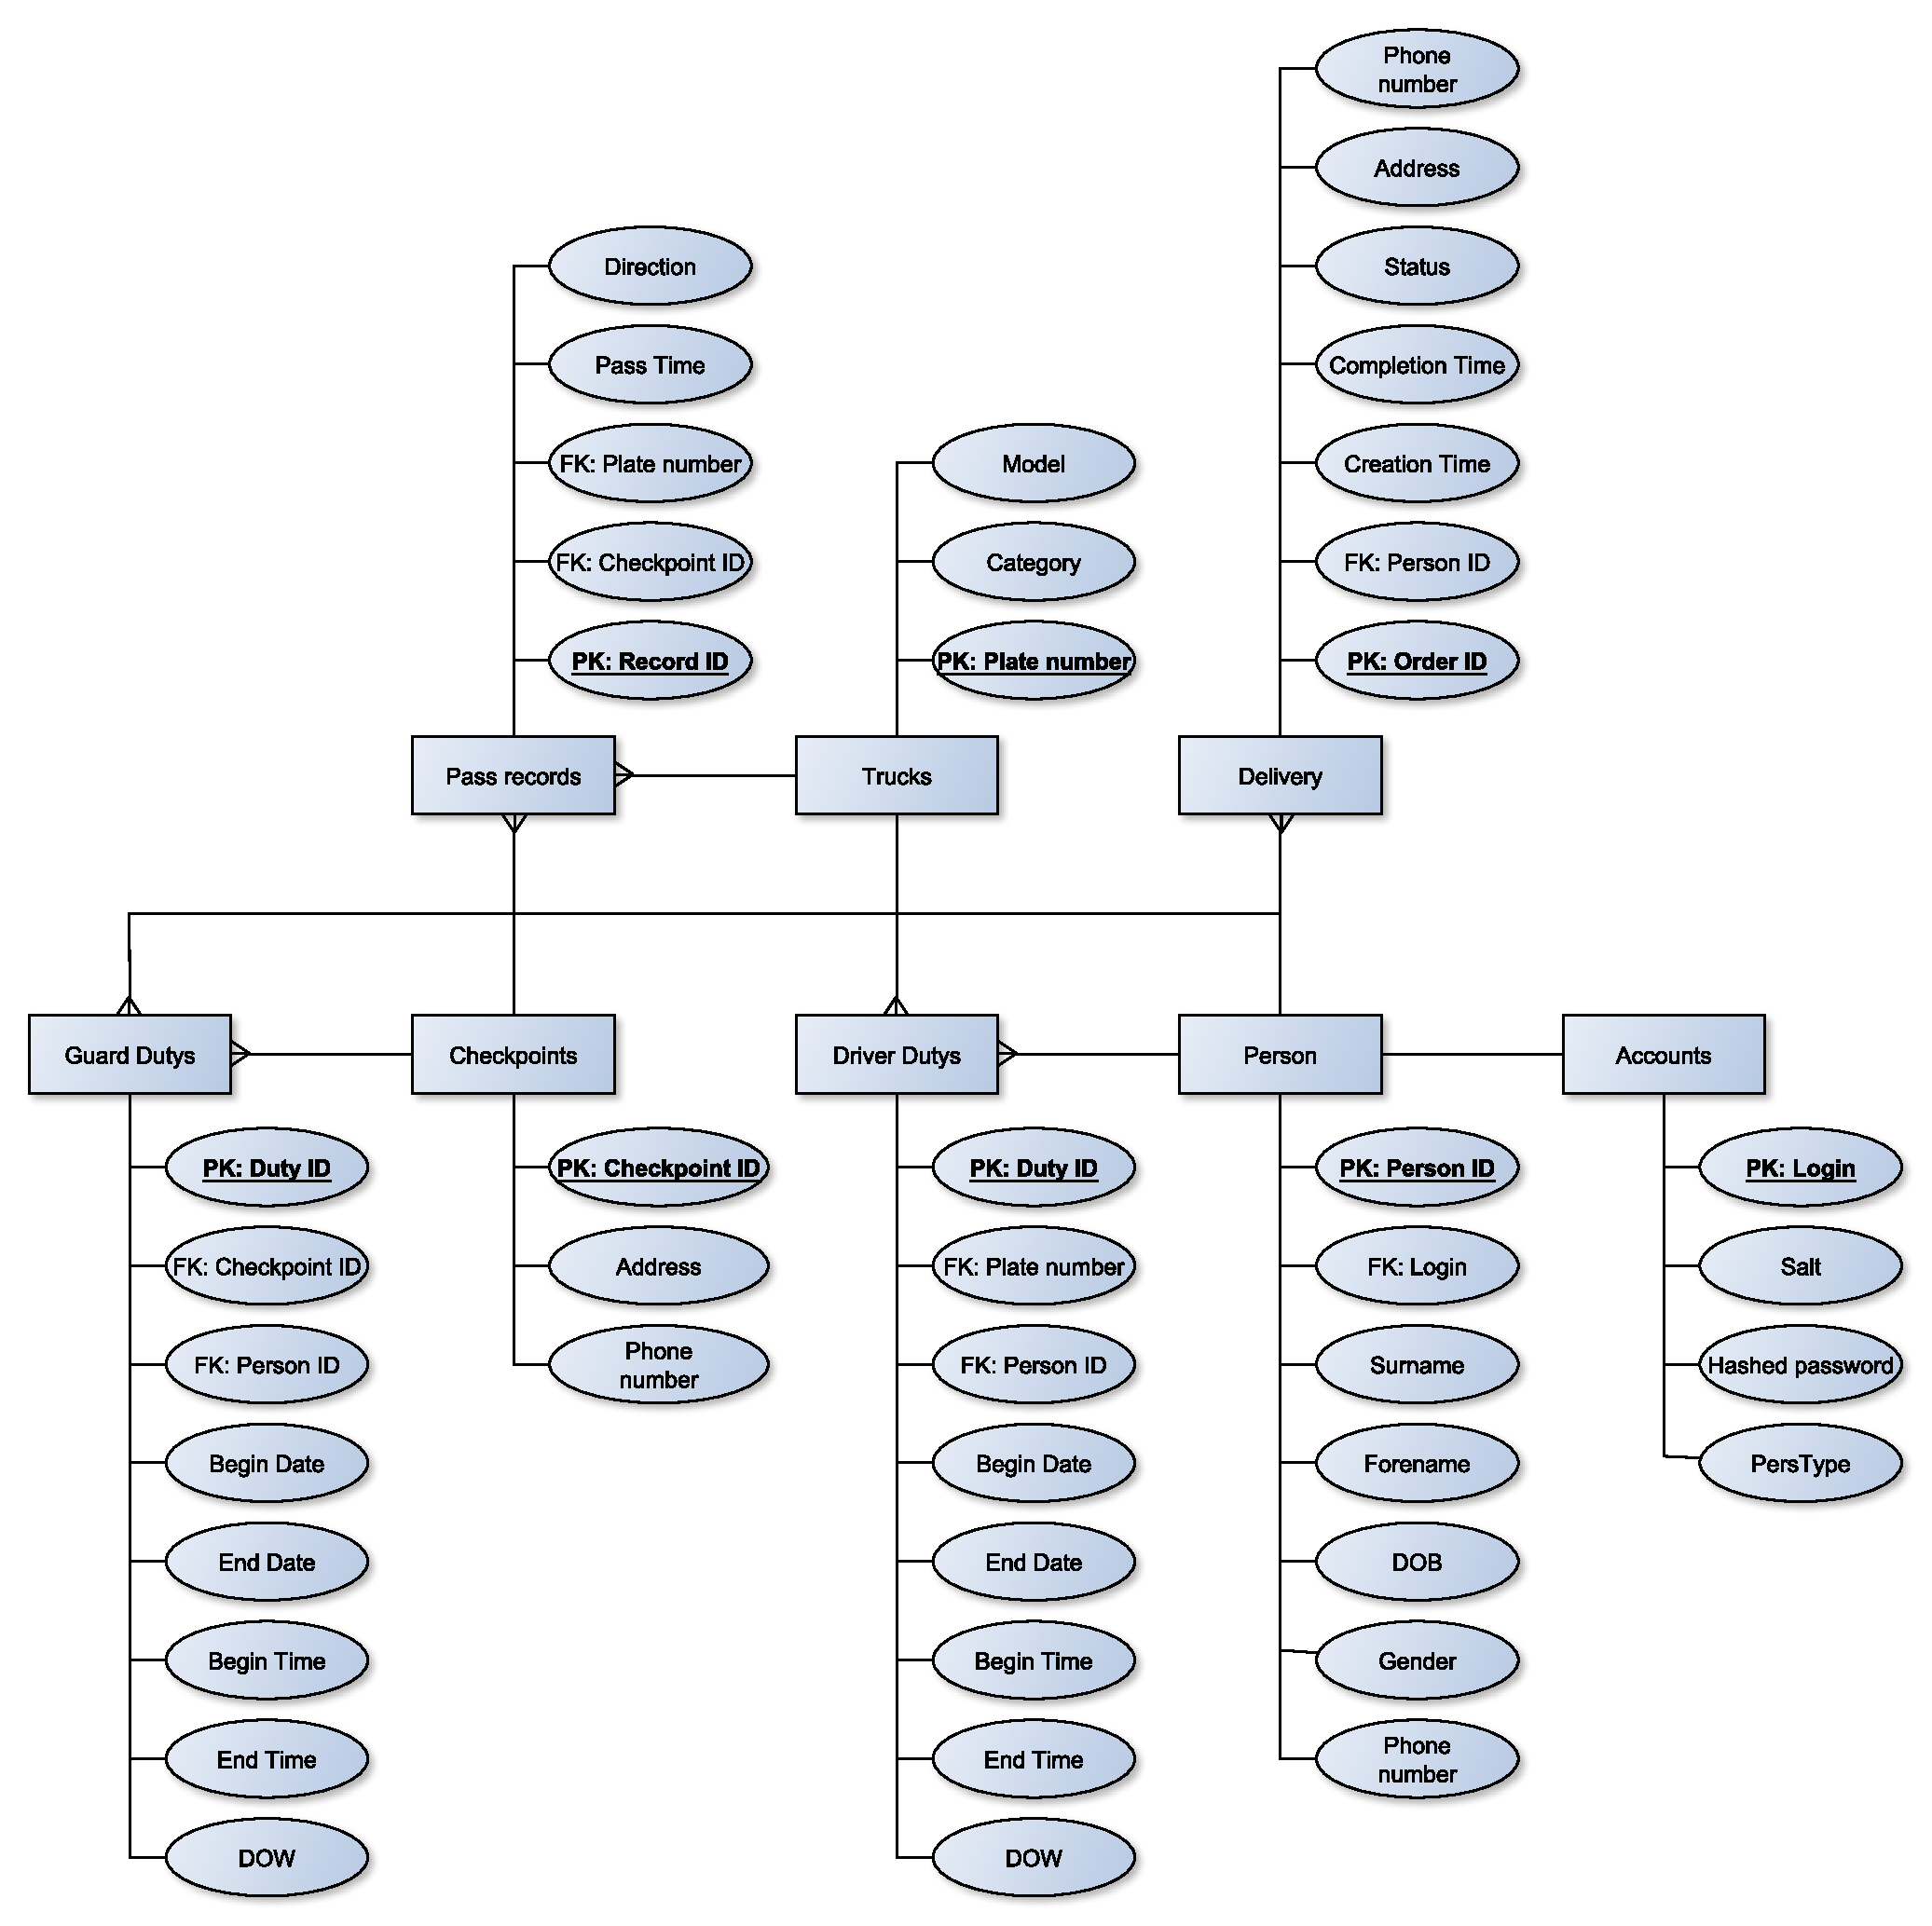
\includegraphics[height=14cm, width = 15cm]{schemes/er_db.pdf}}
			{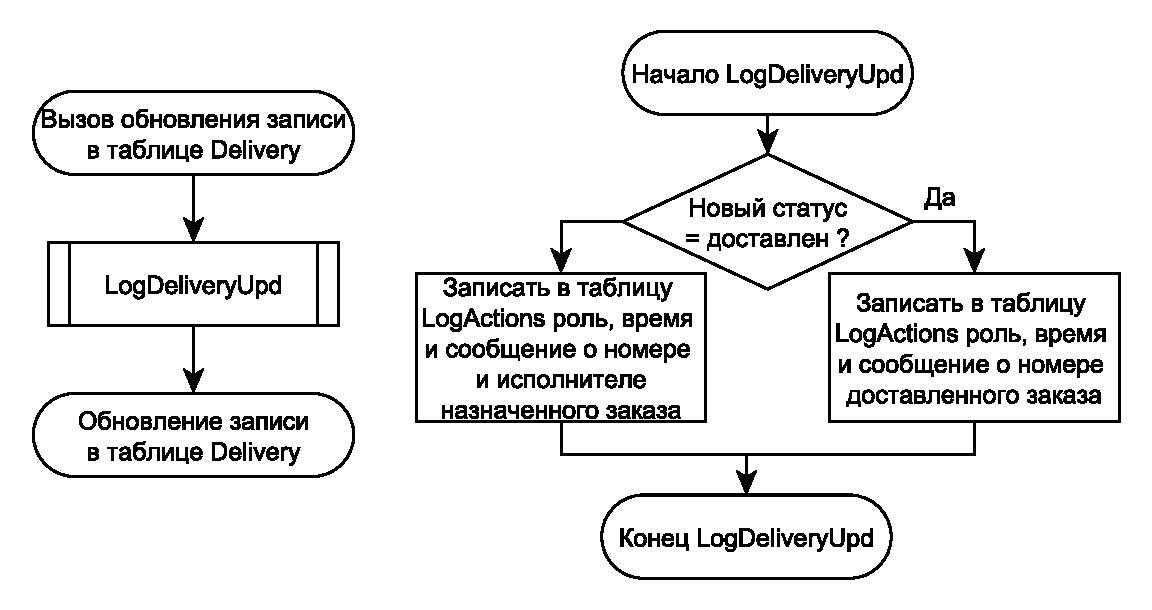
\includegraphics[scale=0.4, angle=0]{sql_schemes/del}}
			\caption{Схема алгоритма триггера на обновление в таблице Delivery}
			\label{del_trig}
		\end{center}
	\end{figure}
\end{itemize}


Также в системе нельзя допускать удаление аккаунтов действующих сотрудников, так как с ними связанна некоторая информация. Например, для доставленных заказов обязательно требуется хранить информацию о его курьере. Поэтому также был создан триггер на удаление записей из таблицы Accounts, запрещающий удалять сотрудников с активным статусом. Схема данного триггера представлена на рисунке \ref{acc_trig}
\begin{figure}[h!]
	\begin{center}
		%			{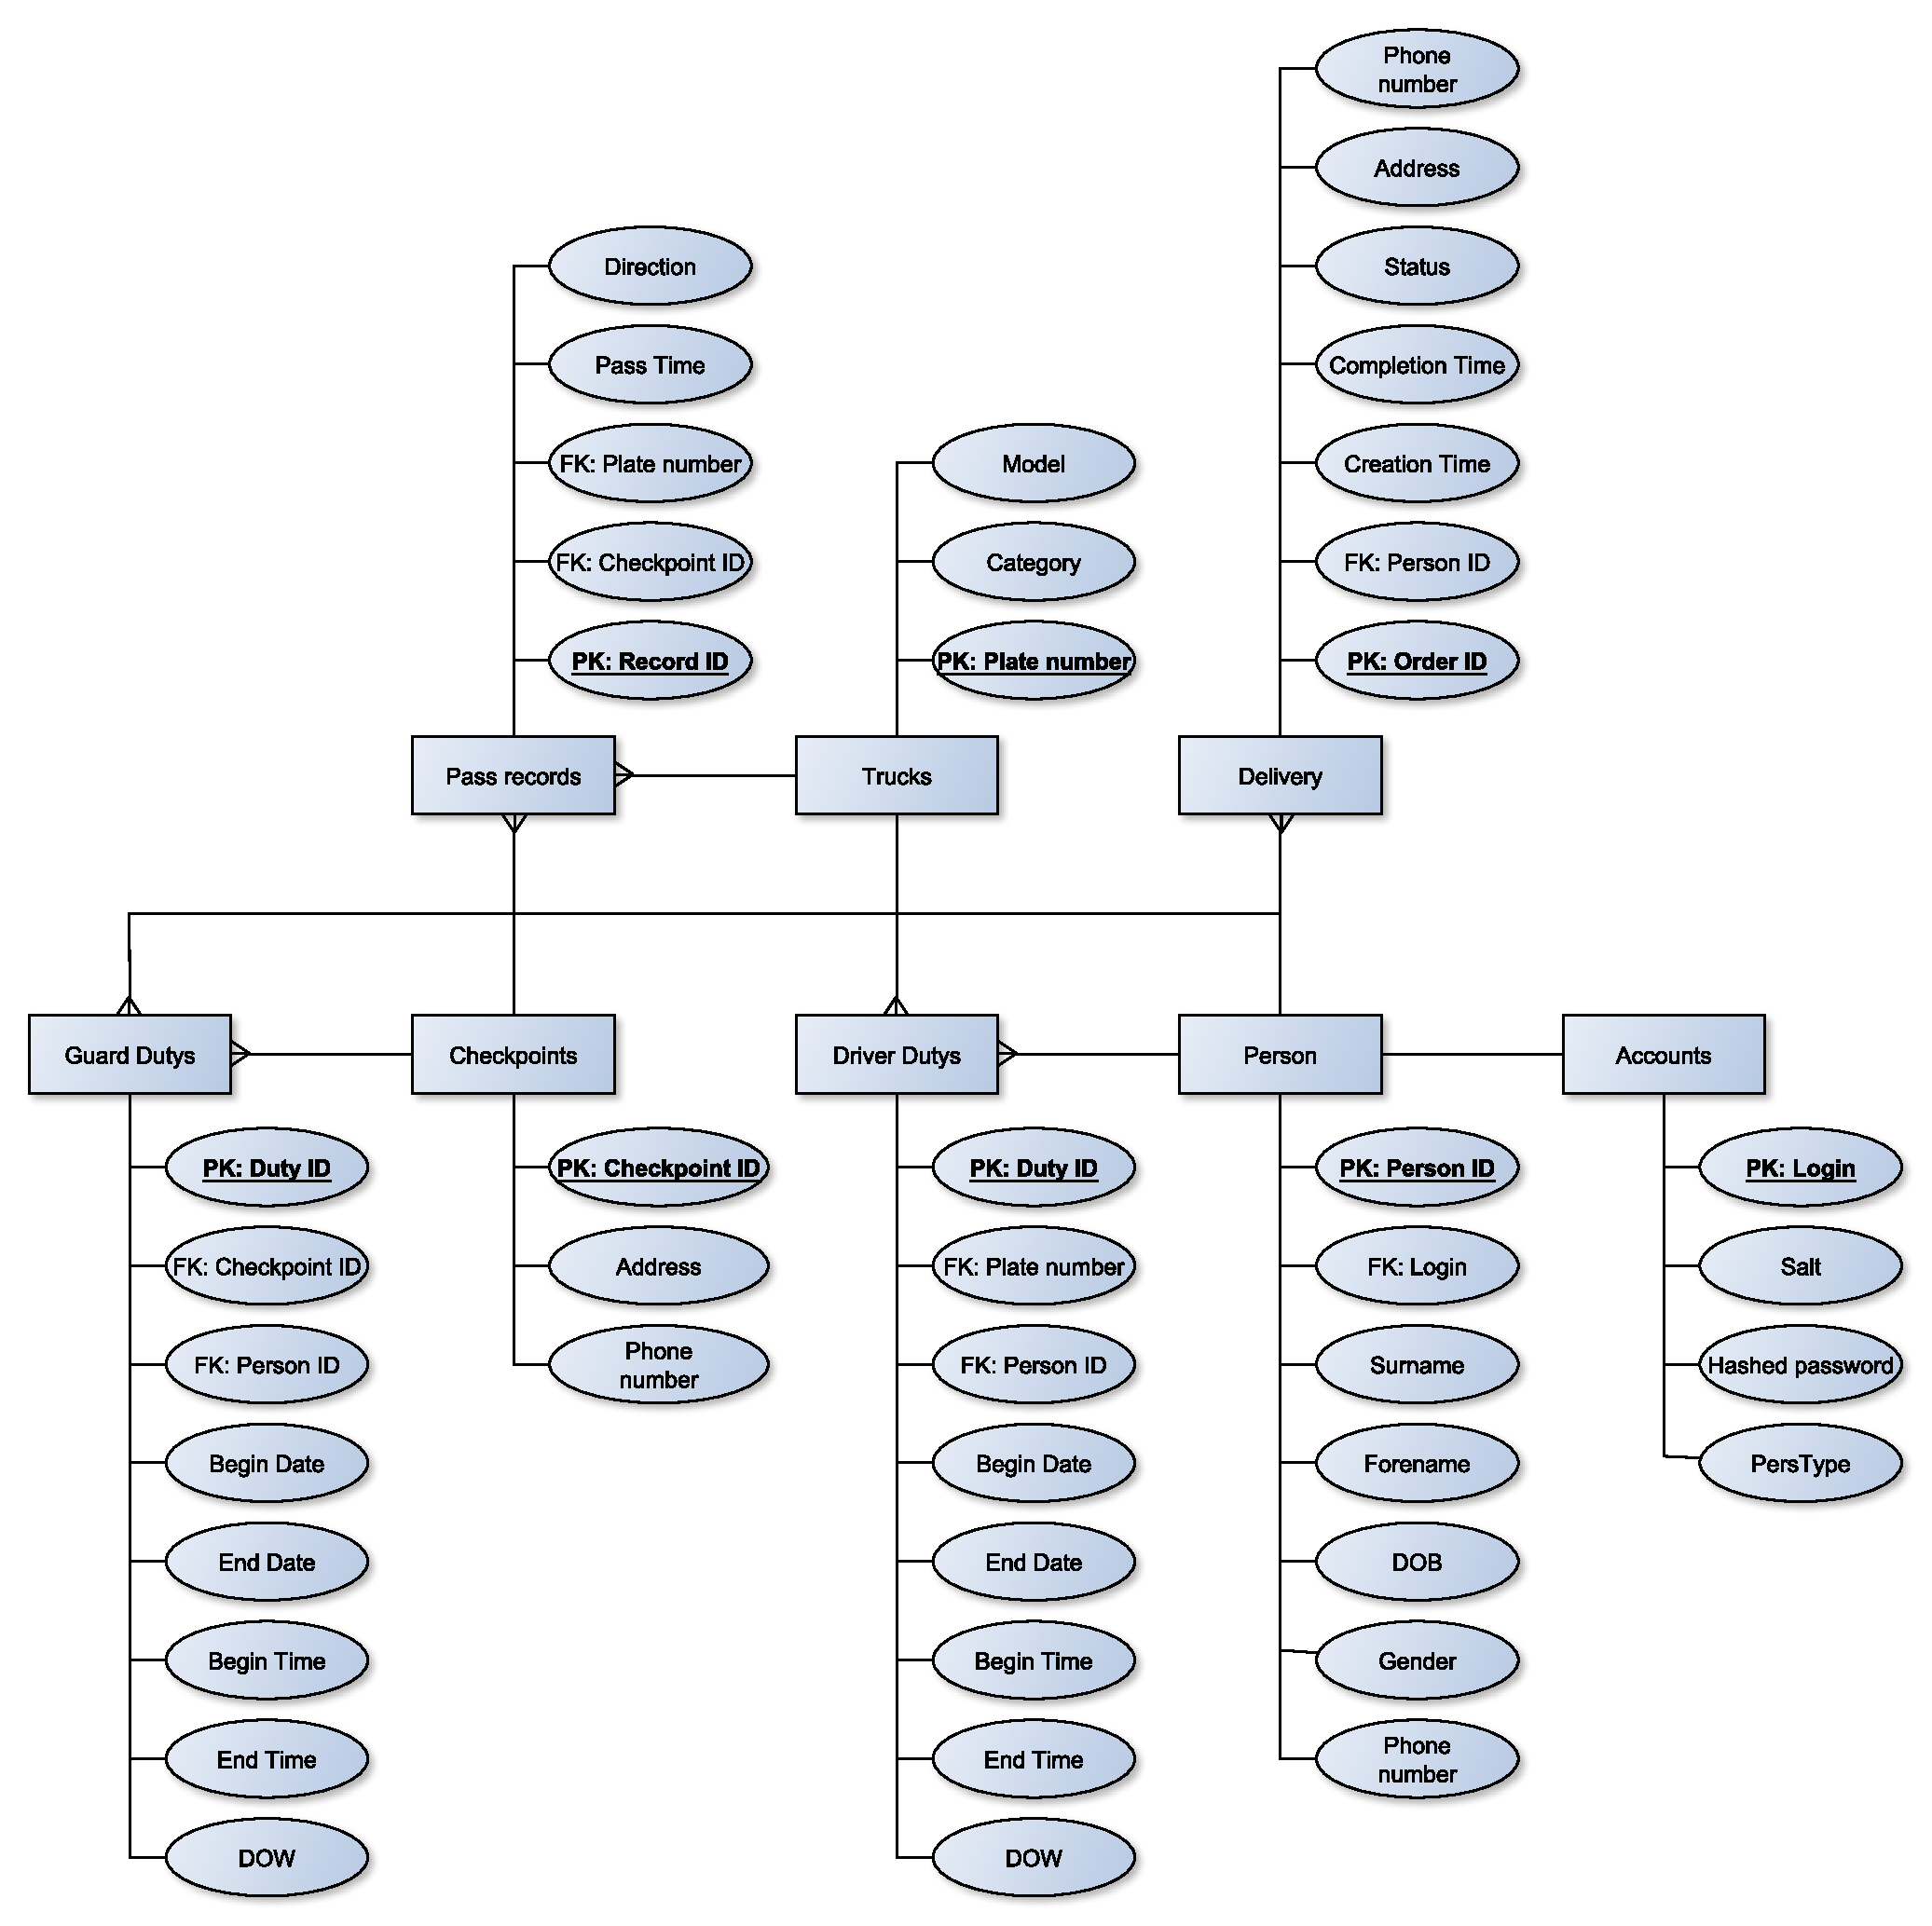
\includegraphics[height=14cm, width = 15cm]{schemes/er_db.pdf}}
		{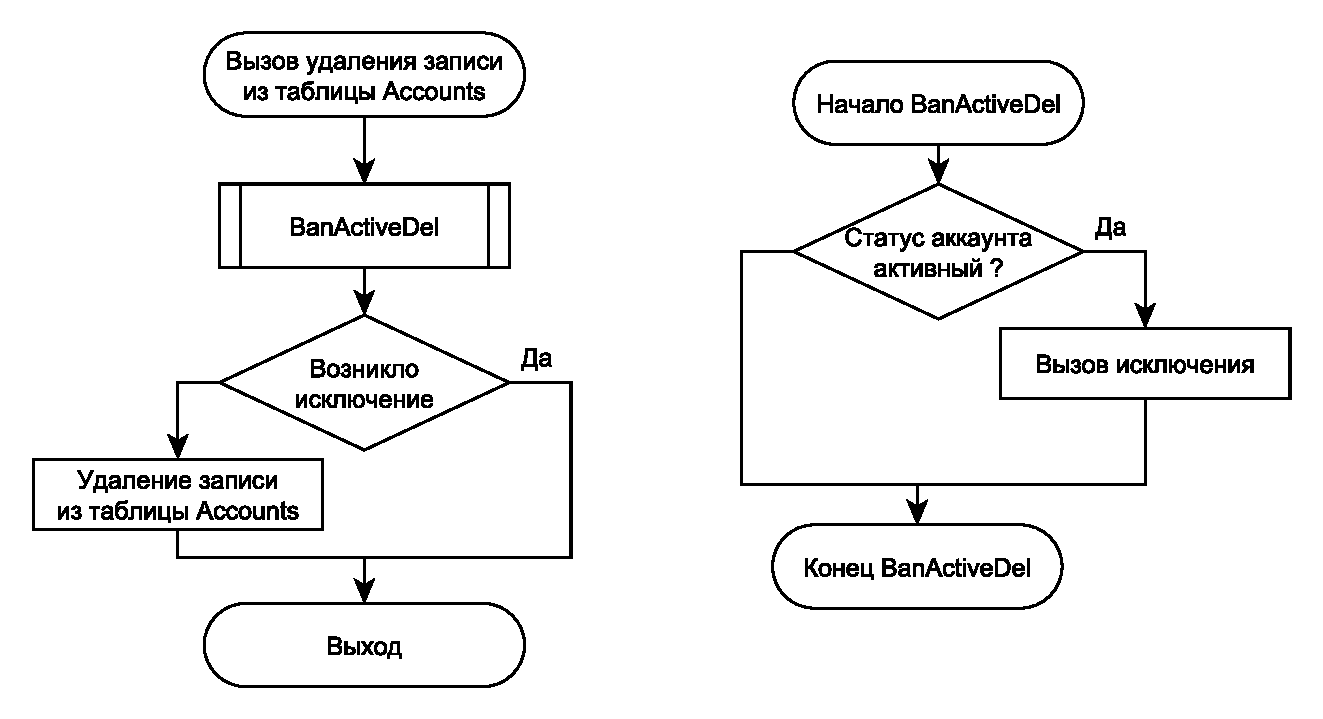
\includegraphics[scale=0.4, angle=0]{sql_schemes/acc}}
		\caption{Схема алгоритма триггера на удаление из таблицы Accounts}
		\label{acc_trig}
	\end{center}
\end{figure}


\section{Архитектура приложения}
Наиболее известным подходом к проектированию архитектуры web-приложения является шаблон MVC. Данный паттерн предполагает разделение приложения на три описанные части.
\begin{itemize}
	\item Model (модель) - компонент бизнес-логики, отвечает за взаимодействие с базой данной и основную обработку информации.
	\item View (представление) - компонент, отвечающий за отображения данных, полученных в результате работы модели.
	\item Controller (контроллер) - компонент, отвечающий за получение запроса от пользователя, передачу их модели для дальнейшего обновления представления.
\end{itemize}

В данной курсовой работе будет использован описанный подход, так как он чётко разграничивает зоны каждого компонента, что позволяет сделать их независимыми.


\section*{Вывод}
Результатом конструкторской части стала разработка сценариев использования приложения, его архитектуры и проектирование таблиц и триггеров базы данных.



